\section{Theoretische Grundlagen}

\subsection{Übersicht über Large Language Models (Sebastian Viet)}

Large Language Models (LLMs) stellen ein bedeutendes Forschungsfeld innerhalb
der künstlichen Intelligenz (KI) dar. Sie basieren auf komplexen neuronalen
Netzwerken, die auf die Generierung und Verarbeitung natürlicher Sprache
spezialisiert sind, und gehören zur Klasse der Foundation Models. Bekannte
Beispiele hierfür sind ChatGPT (OpenAI), Llama (Meta), Bard (Google) oder
DeepSeek (Lian Wenfeng). Insbesondere Unternehmen zeigen großes Interesse an
der Nutzung dieser Modelle, da sie ein erhebliches Potenzial zur Steigerung
der Produktivität bieten. Der aktuelle Trend zeigt, dass LLMs zunehmend in
bestehende Software integriert oder bei Neuentwicklungen unmittelbar
berücksichtigt werden \autocites[Vgl.][S. 1-2,5]{lu2024taxonomy}[S. 1-2]{minaee2024survey}

Das Training von LLMs erfolgt auf Basis des Generative Pretrained
TransformerAnsatzes (GPT). Durch Mechanismen wie Gewichtung (Attention) und
SelfSupervised Learning wird die Vorhersage des nächsten Tokens ermöglicht.
Die zugrunde liegenden Trainingsdatensätze umfassen oft mehrere Petabytes, was
den Modellen erlaubt, trotz breiter Themenvielfalt komplexe Zusammenhänge zu
erkennen. Darüber hinaus entwickeln LLMs emergente Fähigkeiten wie In-Context
Learning oder MultiStep Reasoning \autocites[Vgl.][S. 6-10]{lu2024taxonomy}{lu2024taxonomy}[S. 1-2]{minaee2024survey}[S. 1-2]{naveed2024overview}.

Aufgrund der hohen Anzahl an Parametern und der großen Datenmengen erfordern
sowohl das Training als auch der Betrieb von LLMs erhebliche Rechenressourcen.
Zur Reduzierung dieser Anforderungen werden für spezifische Anwendungsbereiche
Small Language Models (SLMs) entwickelt. Diese Modelle sind weniger
ressourcenintensiv und neigen zu geringeren Halluzinationen, sofern die
Gesprächsthematik mit ihrer trainierten Spezialisierung übereinstimmt. Ein
weiterer vielversprechender Ansatz besteht darin, Halluzinationen zunächst
durch ein SLM zu identifizieren und anschließend mithilfe eines nachgelagerten
LLMs sowie dessen Constraint-Based Reasoning-Funktion hinsichtlich Konsistenz
und Logik zu verbessern. Huang, Yu, Ma et al. betonen, dass die Bereitstellung
verfeinerter Halluzinationskategorien es LLMs ermöglicht, Halluzinationen
zuverlässiger zu erkennen \autocites[Vlg.][]{kelbert2023llm}{huang2024hallucination}[S. 6-14]{hu2024slm}

\subsection{Effizienzoptimierung (Sebastian Viet)}

Bei Pruning handelt es sich um eine Methode zur Reduktion der Komplexität und
Größe bei Modellen. Sie findet Anwendung im Bereich der Entscheidungsbäume und
neuronalen Netzen. Die Effizienzsteigerung wird durch die Entfernung
irrelevanter Teile erzielt. Pruning kann in drei Unterkategorien unterteilt
werden: strukturelles, unstrukturelles und adaptives Pruning. Diese werden
folgend weiter vorgestellt. Der Schwerpunkt wird auf strukturelles Pruning
gelegt, da dieses auch später im Praxisteil Anwendung findet.

Das Kapitel wird durch die Vorstellung einer weiteren Unterscheidungsvariante
aus einer Metastudie von Vadera und Ameen abgerundet.

\subsubsection{Strukturelles Pruning}

Beim strukturellen Pruning werden ganze Teileinheiten wie Filter oder Kanäle
aus dem neuronalen Netz entfernt. Die Modelle werden kompakter und dadurch auch
auf Standardhardware ausführbar. Ebenso die gute Kompatibilität zu
Standardbibliotheken aus dem Deep Learning-Segment und die Möglichkeit das
Pruning mit weiteren Kompressionsverfahren zu kombinieren, machen den Ansatz
attraktiv. Beides wirkt sich positiv auf die entstehenden Kosten aus.
\autocites[Vgl.][S. 1]{he2023structured}[S. 1-2]{vadera2022methods}

Die Ausgangslage ist ein bereits trainiertes Netz. Die Herausforderung beim
Pruning ist die Identifizierung der Teileinheiten, die ohne Verlust an
Modellgenauigkeit löschbar sind. Zum einen kann die Selektion gewichtsabhängig
erfolgen. Hierfür werden z.B. anhand des geometrischen Medians redundante
Filter identifiziert. Alternativ ist eine Betrachtung der L1-Norm (Summe aller
Absolutwerte eines Vektors) und L2-Norm (Quadratwurzel der Summe der Quadrate
der Einträge eines Vektors) möglich. Filter mit kleinen Summen werden entfernt.
Hierbei spricht man von magnitudenbasierten Metriken. Neben der Betrachtung
der Gewichte kann auch die Aktivierung als Kriterium genutzt werden. Der
Rekonstruktionsfehler, der durchschnittliche Rang oder die Anzahl an Nullen
auf den Aktivierungskarten werden als Kriterien für die Eliminierung genutzt.
Über eine Kreuzkorrelation kann zudem die Unabhängigkeit eines Kanals bestimmt
werden. Mit der Taylor-Expansion kann der entstehende Verlustwert nach
Entfernung eines Filters möglichst annähernd ermittelt werden. He und Xian
ordnen die Taylor-Expansion der Unterkategorie optimierungsbasierten Methoden
zu, während Vadera und Ameen den Ansatz zur Gruppe der Sensitivity Analysis
zählen. Unabhängig von der gewählten Methode ist es wichtig nach der Entfernung
von Strukturen ein Finetuning vorzunehmen. Dieses dient dazu die Leistung zu
optimieren und soll auftretende Genauigkeitsverluste auszugleichen. \autocites[Vgl.][S. 1-5]{he2023structured}[S. 1-5]{vadera2022methods}

\subsubsection{Unstrukturelles Pruning}

Während beim strukturellen Pruning ganze Neuronen, Kanäle oder Filter entfernt
werden, wird beim unstrukturellen Pruning jede Gewichtsverbindung analysiert
und bewertet. Die Zielsetzung besteht erneut darin, überflüssige Informationen
zu entfernen. Die Reduktion führt jedoch zu einer reduzierten Gewichtsmatrix
mit unregelmäßigen Mustern. Die Umsetzung erfolgt meist über
Maskierungstechniken. Diese deaktivieren durch binäre Masken unwichtige
Gewichte. \autocite[Vlg.][S. 3]{cheng2024survey}

Da klassische GPUs auf dichte Matrizen optimiert sind, erfordert der Einsatz
spezielle Hard- und Software. Es handelt sich somit um eine kostenintensivere
Variante als das strukturierte Pruning. Die Bewertung jedes einzelnen Gewichts
lässt zwar eine sehr feine Kontrolle über die Einsparung zu, jedoch kann das
fehlerhafte Entfernen einer einzelnen kritischen Verbindung bereits zu
Informationsverlust führen. Unter sorgfältiger Berücksichtigung dieser Gefahr
kann jedoch ein hoher Kompressionsgrad erzielt werden. So zeigen Zhu und Gupta
mittels Pruning verschiedener neuronaler Architekturen, dass eine Kompression
ohne Leistungsbeeinträchtigung um bis 90\% möglich ist.\autocites[Vgl.][S.3]{cheng2024survey}[S. 6-8]{zhu2022prune}

\subsubsection{Adaptive Pruning Verfahren}

Im Gegensatz zu traditionellen Pruning-Verfahren, bei denen die Kriterien im
Voraus festgelegt werden, erfolgt das adaptive Pruning dynamisch während des
Trainings. Das Verfahren passt sich dynamisch an Änderungen wie Gewichte,
Gradienten oder Aktivierungen an und maximiert so die Effizienz. Manuelle
Anpassungen werden auf ein Minimum beschränkt. Auch die komplexe Ermittlung
von Parametern, die universell für das vollständige Modell gelten könnten,
entfällt. Wie beim unstrukturierten Pruning muss die Hardware jedoch sparse
Matrizen verarbeiten können. Im Gegenzug ist adaptives Pruning sehr flexibel
und somit ideal für ressourcenbegrenzte Geräte. Beispielsbereiche sind das
autonome Fahren sowie moderne Smartphones und Tablets mit dedizierten KI-Chips.

Prominente Beispiele sind das Layer-Adaptive-Pruning oder das Adaptive
Channel-Pruning. Ersteres leitet die unterschiedlichen Pruning-Raten je Schicht
aus der Sensitivität ab. Letzteres arbeitet mit der Entfernung von Kanälen in
CNNs. \autocites[Vgl.][S. 295-296]{sakai2022structured}[S. 1-2]{wang2025adapt}


\subsubsection{Weitere Möglichkeiten der Kategorisierung von Pruning}

In einer Metastudie haben Vadera und Ameen über 150 Paper zu Pruning
untersucht. Hierbei gruppierten sie die Veröffentlichungen nicht nach
strukturiert, unstrukturiert und adaptiv, sondern nach dem verwendeten
(mathematischen) Ansatz. Es konnten acht Kategorien gebildet werden, die kurz
benannt und vorgestellt werden:\autocite[Vgl.][S. 2]{vadera2022methods}

\begin{itemize}
	\item \textbf{Magnitude-based Pruning Methods:} Relevanz von Gewichten und Neuronen wird über lokale Maße wie z. B. die Magnitude bestimmt.
	\item \textbf{Similarity and Clustering Methods:} Identifizierung und Entfernung redundanter oder sehr ähnlicher Gewichte.
	\item \textbf{Sensitivity Analysis Methods:} Entfernung der Gewichte, die geringen Einfluss auf das Endergebnis haben.
	\item \textbf{Knowledge Distillation Methods:} Ableitung eines neuen Modells („Student“) aus dem Ursprungsmodell („Teacher“).
	\item \textbf{Low-Rank Methods:} Zerlegung der Gewichtsmatrix in ein Produkt aus zwei kleineren Matrizen.
	\item \textbf{Quantization Methods:} Verwendung von Hashing, niedriger Präzision oder binärer Darstellung, um die Berechnungsaufwände zu reduzieren.
	\item \textbf{Architectural Design Methods:} Nutzung von Such- und Reinforcement-Learning zur Erstellung neuronaler Netzwerkarchitekturen.
	\item \textbf{Hybrid Methods:} Kombination mehrerer Ansätze zur Steigerung der Kompressionseffekte.
\end{itemize}

Erwähnenswert ist zudem, dass diese acht Kategorien teilweise noch feiner
unterteilt werden konnten. Abbildung 1 zeigt eine Auswahl aus den ersten drei
Kategorien der Metastudie.

\begin{figure}[H]
	\centering
	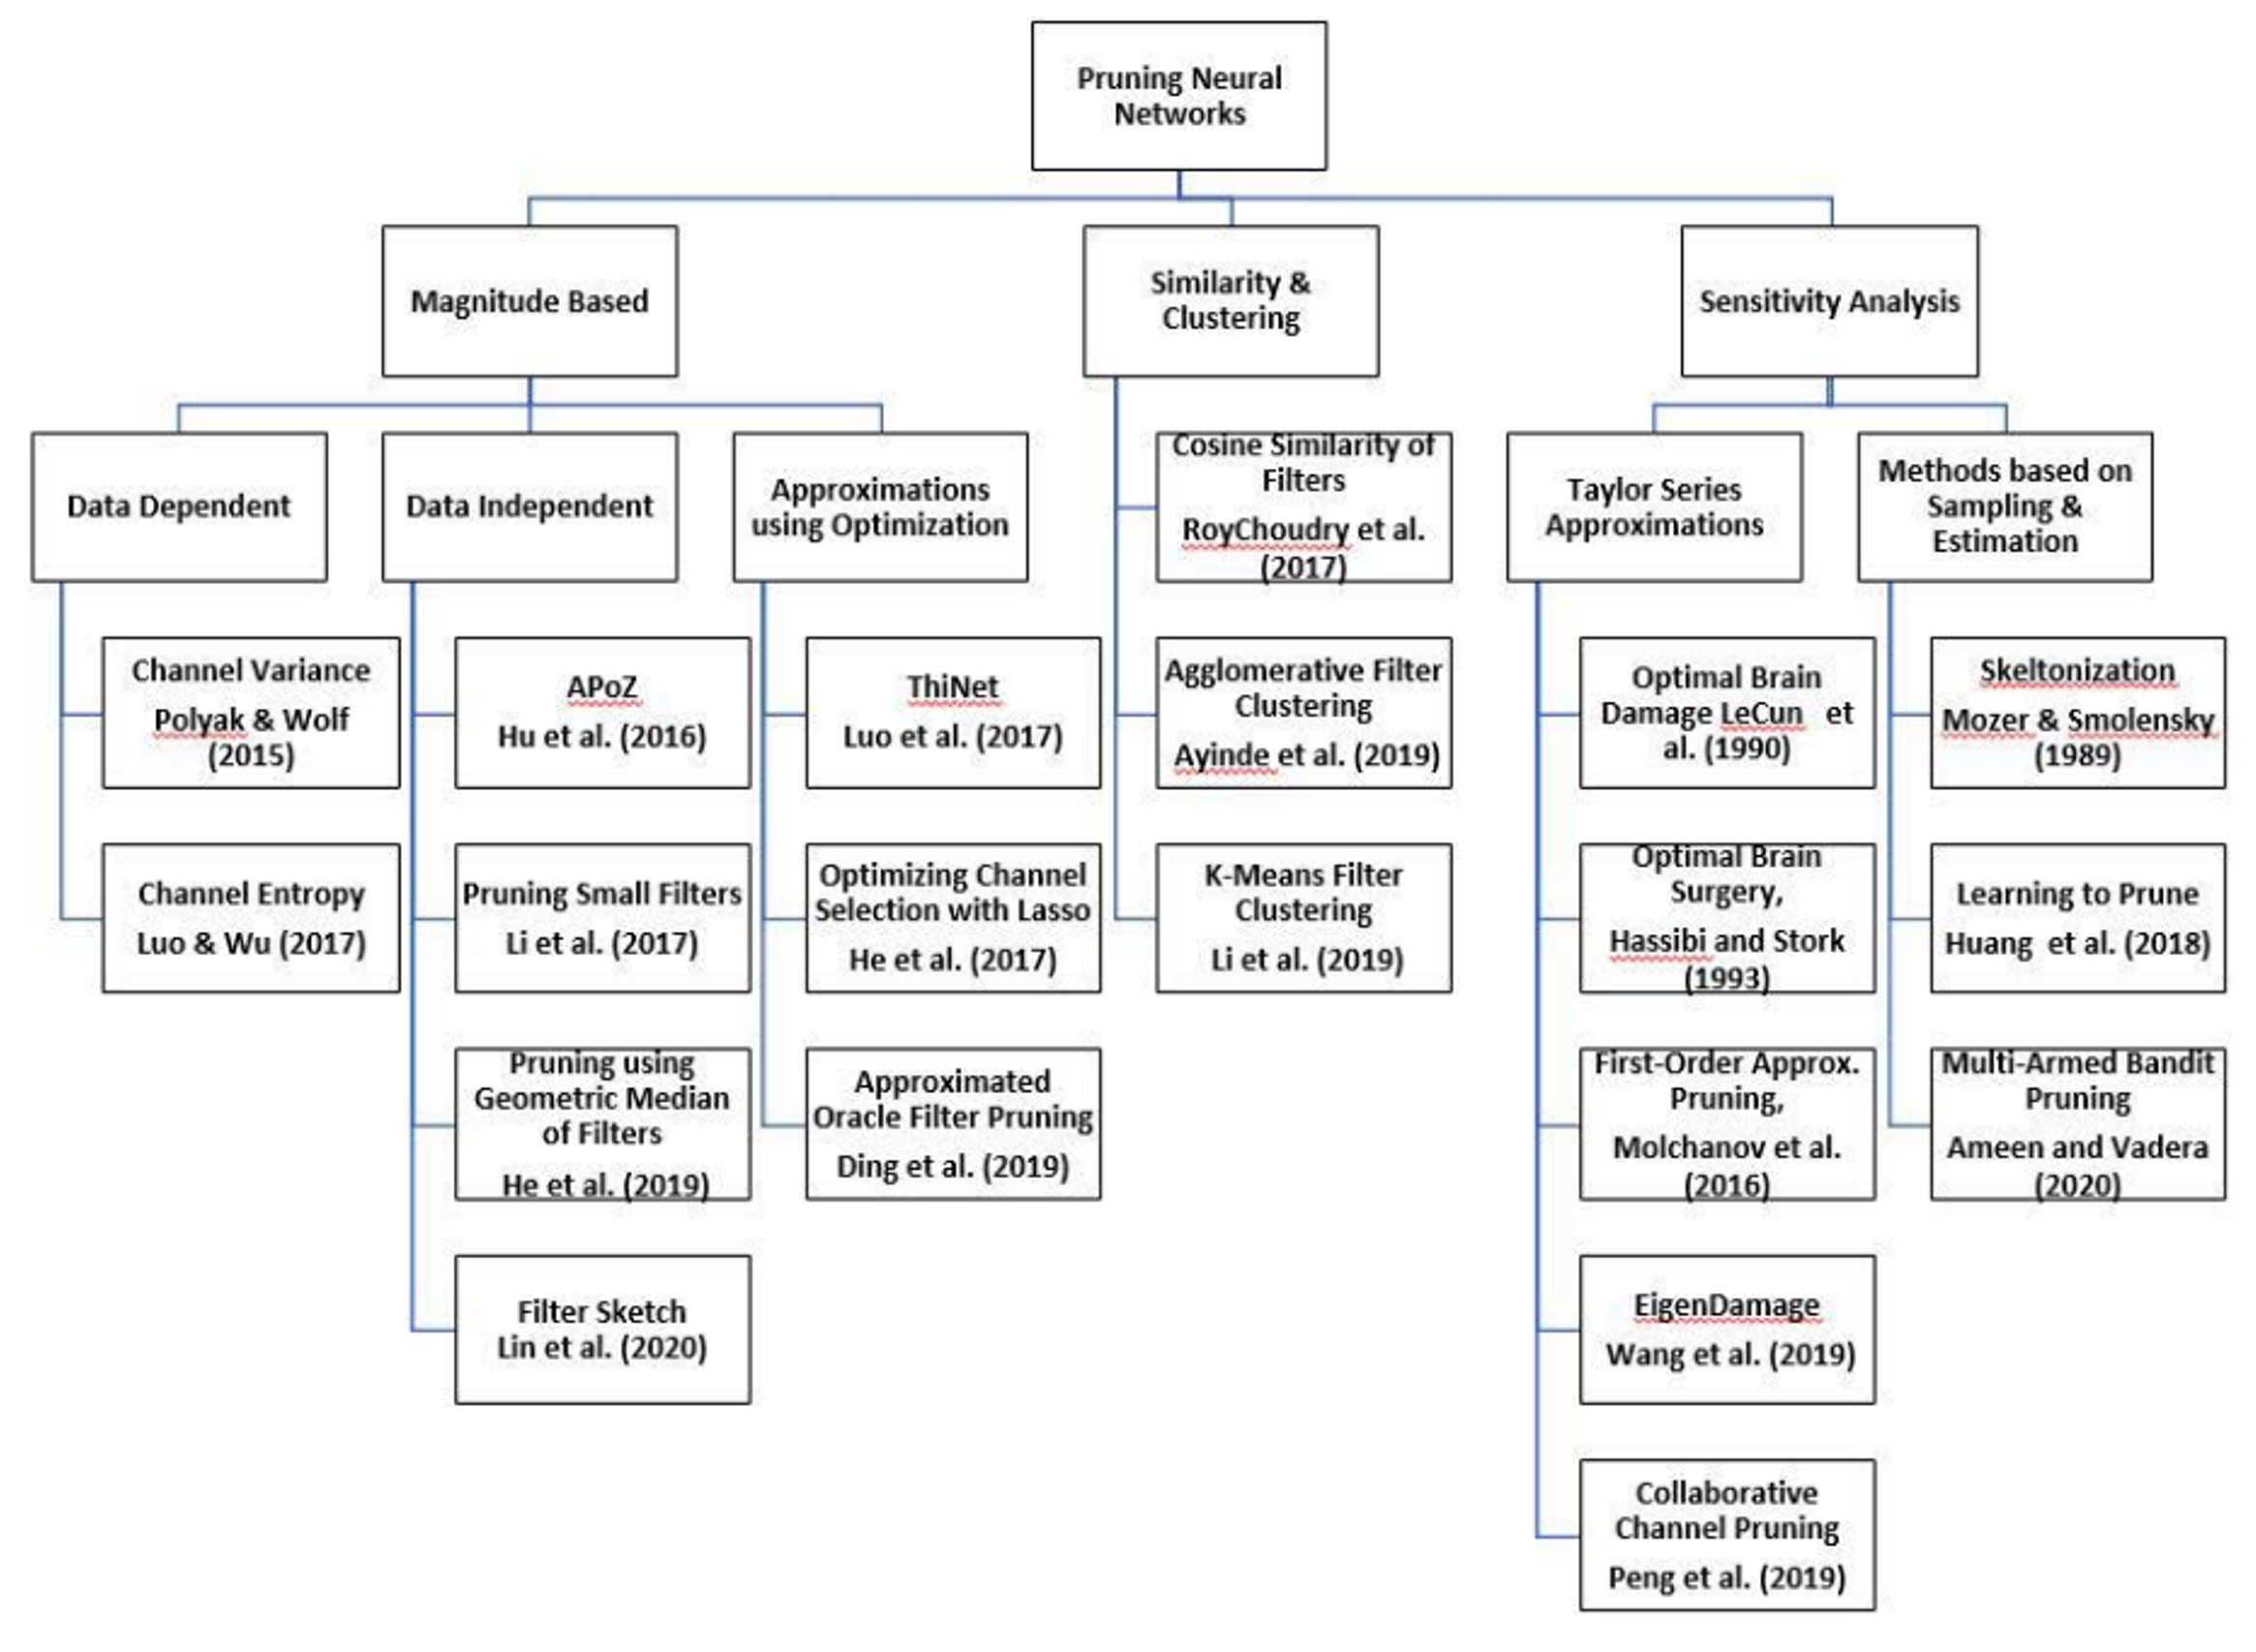
\includegraphics[width=0.9\textwidth]{images/pruning.png}
	\caption[Pruning-Methoden nach Vadera und Ameen]{Aufteilung nach Vadera und Ameen\\Quelle: \cite{vadera2022methods}}
	\label{fig:vadera}
\end{figure}

\subsection{Frameworks (Kai Herbst)}

\subsubsection{LLM-Pruner}

In dieser Arbeit wird das \emph{LLM-Pruner}-Framework verwendet. Das Framework
stellt einen strukturellen Ansatz zum Pruning von LLMs dar, das die
Multi-Tasking-Fähigkeiten der Modelle weitestgehend erhalten soll und im
Vergleich mit anderen Frameworks deutlich schneller arbeitet. Die
Multi-Tasking-Fähigkeit soll dabei erhalten bleiben, indem der \emph{LLM-Pruner}
ohne aufgabenspezifisches Feintuning auskommt. Im Andere Frameworks verwenden im
Gegensatz dazu Methoden zur Modellkomprimierung, die sich darauf konzentrieren,
ein Modell für eine bestimmte Aufgabe zu optimieren.\autocite[Vgl.][]{llmpruner}

Wie bereits erwähnt, arbeitet der \emph{LLM-Pruner} mit einem strukturellen
Pruning. Dabei werden zusammenhängende Modellstrukturen analysiert und nur die
weniger wichtigen entfernt, sodass der Kern des Modells möglichst erhalten
bleibt. Der Prozess läuft in drei Schritten ab:

\begin{itemize}
	\item \emph{Dependency Discovery}: Zunächst wird untersucht, welche Teile
	      des Modells stark miteinander verbunden sind, sodass nichts entfernt
	      wird, das für die Modellarchitektur essenziell ist.

	\item \emph{Importance Estimation}: Anschließend wird bewertet, welche
	      Komponenten besonders wichtig für die Gesamtleistung des Modells sind –
	      basierend auf Gradienten- und Hessian-Informationen.

	\item \emph{Fast Recovery mit LoRA}: Schließlich wird das geprunte Modell
	      mithilfe von Low-Rank Approximation (LoRA) nachtrainiert, um mögliche
	      Leistungseinbußen zu minimieren.
\end{itemize}

Im Paper des \emph{LLM-Pruners} wird damit geworben, bei einer Reduktion von
20\% immer noch rund 95\% der ursprünglichen Performance beibehalten zu können.

\subsubsection{Wanda}

Ein weiteres mögliches Framework, das aufgrund technischer Probleme nicht im
praktischen Teil der arbeit zum Einsatz gekommen ist, ist \emph{Wanda} (Pruning
by Weights and Activation), dessen dazugehöriges Paper "A Simple and Effective
Pruning Approach for Large Language Models" auf der ICLR 2024 veröffentlicht
wurde. Das Besondere hierbei ist, dass diese Pruning-Methode ohne Retraining,
also ohne nachträgliches Training des Modells gute Resultate erzielen
soll.\autocite[Vgl.][]{wanda}

Die Wanda-Methode basiert auf der Beobachtung, dass in LLMs einige
Aktivierungswerte außergewöhnlich hoch sind. Statt Gewichte nur anhand ihrer
absoluten Werte zu bewerten, wie man es bei den magnitudenbasierten Verfahren
der Fall ist, kombiniert Wanda die Gewichtsmagnitude mit der Norm der
zugehörigen Aktivierungen. So werden jene Gewichte entfernt, die den geringsten
Einfluss auf die Modellleistung haben.

\subsection{Bewertungskriterien (Sebastian Viet)}

Um die Effizienz der unterschiedlichen Pruning-Ansätze zu ermitteln, ist das
Heranziehen des Random-Pruning als Vergleichsmethode beliebt. Li, Adamczewski
et al. unterscheiden dabei in drei verschiedene Wege, wie das Random-Pruning
umgesetzt werden kann:

\begin{itemize}
	\item \textbf{Vollständig zufällig:} Das Pruning findet zufällig und ohne weitere Vorgaben statt.
	\item \textbf{Eingeschränkt zufällig:} Das Pruning-Verhältnis wird je Schicht vorgegeben. Innerhalb der Schicht erfolgt das Pruning jedoch weiterhin zufällig.
	\item \textbf{Zufällige Kanalanzahlauswahl:} Das Pruning-Verhältnis wird je Schicht zufällig ausgewählt.\autocite[Vgl.][]{li2022random}
\end{itemize}

Sowohl He und Xiao als auch Li, Adamczewski et al. konstatieren in ihren
Untersuchungen ein überraschend gutes Abschneiden des Random-Prunings im
Vergleich zu weiterentwickelten Methoden.\autocites[Vgl.][]{he2023structured}{li2022random}

Relevanter ist jedoch die Frage, inwieweit das Sprachmodell nach dem Pruning
noch „funktionsfähig“ ist. Hierunter wird die Fähigkeit verstanden Eingaben in
das Modell auf plausible Weise zu beantworten. Zur Untersuchung kommen extra
auf diese Fragestellung zugeschnittene Benchm (Sebastian Viet)arks zum Einsatz. Diese enthalten
Testfragen, welche an das Sprachmodell gestellt werden, sowie zugehörige
Lösungen, die mit den Antworten des LLMs in Anschluss abgeglichen werden. Bei
der Auswahl des Benchmark-Modells ist auf dessen Prüfziele zu achten. So
unterscheiden sich die Modelle im Schwierigkeitsgrad und in der Breite der
Themenabfrage. Die im Projekt eingesetzten Benchmark-Modelle werden im
Folgenden kurz vorgestellt.


\begin{itemize}
	\item \textbf{BoolQ (Boolean Questions):} Der Datensatz enthält 15.942 Ja-/Nein-Fragen. Die Fragen sind realen Kontexten entnommen und nicht generiert worden. Neben der Fragestellung wird dem LLM ein Begleittext mitgegeben, welcher die Antwort auf die Frage bzw. Hilfestellungen enthält. Hierbei wird jedoch oft auf komplexere Schlussfolgerungen durch die KI gesetzt. Als einfaches Beispiel zum Verständnis sei folgender Begleittext gegeben: Spanien hat die Fußball-EM 2024 gewonnen. Die zugehörige Frage lautet: Hat Harry Kane die EM 2024 gewonnen? Die KI muss nun trotz ihres reduzierten neuronalen Netzes erkennen, dass Harry Kane zwar ein Fußballspieler ist, aber als Nationalspieler für England und nicht für Spanien im Finale antrat. Die Antwort muss daher Nein lauten.\autocite[Vgl.][S. 1-2]{clark2019boolq}

	\item \textbf{Arc-C (AI2 Reasoning Challenge):} Der Datensatz enthält 7.787 Multiple-Choice-Fragen aus dem naturwissenschaftlichen Bereich auf amerikanischem Grundschulniveau (Klassen 3 bis 9). 2.590 der Fragen werden als besonders herausfordernd klassifiziert. Sie gelten als nicht beantwortbar für abrufbasierte oder Wort-Koexistenz-Algorithmen. Optional wird ein Datensatz mit 14 Millionen wissenschaftlichen Sätzen angeboten, welcher der KI zur Beantwortung der Fragen als Hilfestellung gereicht werden kann.\autocite[Vgl.][S. 1]{clark2019arc}

	\item \textbf{HellaSwag:} Bei HellaSwag handelt es sich um die Weiterentwicklung von Swag. Der Datensatz enthält 39.905 Trainingsdatensätze und 5.021 Datensätze für Test und Validierung. Bei HellaSwag ist für das LLM die Aufgabe, einen gegebenen Satz sinnvoll fortzusetzen. Dem LLM werden dabei 4 mögliche Fortsetzungen angeboten, wovon nur eine richtig ist. Das LLM wird somit auf richtige Schlussfolgerungen basierend auf Alltagswissen getestet. Die drei falschen Antwortmöglichkeiten wurden mittels des Adversarial-Filtering-Verfahrens generiert. Auf Basis von iterativ eingesetzten Diskriminatoren werden die negativen Antworten so gestaltet, dass sie für künstliche Intelligenz schwer zu erkennen sind. Der Mensch hingegen kann die falschen Antworten leicht erkennen.\autocite[Vgl.][S. 1-3]{zellers2019hellaswag}

	\item \textbf{OpenBookQA:} Der Datensatz enthält 5.957 Multiple-Choice-Fragen mit je vier Antwortmöglichkeiten. Wie der Name bereits nahelegt, empfindet der Test Open-Book-Prüfungen nach, bei denen die Prüflinge freien Zugang zu Informationen haben. Das Modell enthält daher zu jeder Frage auch ein \textit{core fact}, welches die unterstützende Wissensquelle imitieren soll. Die Fragen sind so gestaltet, dass eine mehrschrittige Schlussfolgerung unter Einbeziehung von externem Wissen notwendig ist.\autocite[Vgl.][S. 1-2]{mihaylov2018armor}

	\item \textbf{WinoGrande:} Bei WinoGrande handelt es sich um die Weiterentwicklung der Winograd Schema Challenge (WSC). Während das Original nur 273 Aufgaben beinhaltet, setzt die Erweiterung auf 44.000 Problemstellungen. Diese wurden auf Basis von Crowdsourcing erstellt und geprüft. Die Aufgaben sind als \textit{fill-in-the-blank}-Probleme gestellt, wo Pronomen durch ihre richtige Referenz ersetzt werden müssen. Um den Schwierigkeitsgrad anzuheben, wurde zusätzlich AfLite (Adversarial Filtering) angewendet. Dies verhindert die Ausnutzung einfacher Wortassoziationen durch das LLM bei der Beantwortung der Fragen.\autocite[Vgl.][S. 1-3]{sakaguchi2019winogrande}
\end{itemize}

\newpage
